While bar graphs and histograms start giving a sense of the variability in
data, they are limited to showing the dispersion of the data only in 1
dimension; namely the measurements themselves. In their survey of the history
of the boxplot \cite{wickham11} Wickham and Stryjewski trace the evolution of
the boxplot from a difinitive box to amorphous envelopes.  They start by laying out
the core statistics of a boxplot: a box centered at the median (or mean) and
bound by the upper and lower quartiles (termed the hinges), and two whiskers which represent the
extremes (often 1.5 the outer quartiles, sometimes the \alpha bounds). Sometimes there's
also a dot to signify outliers, as seen in \ref{fig:boxplot}, but one of
the strengths of the box plot has been in it's flexibility. 

\begin{figure}
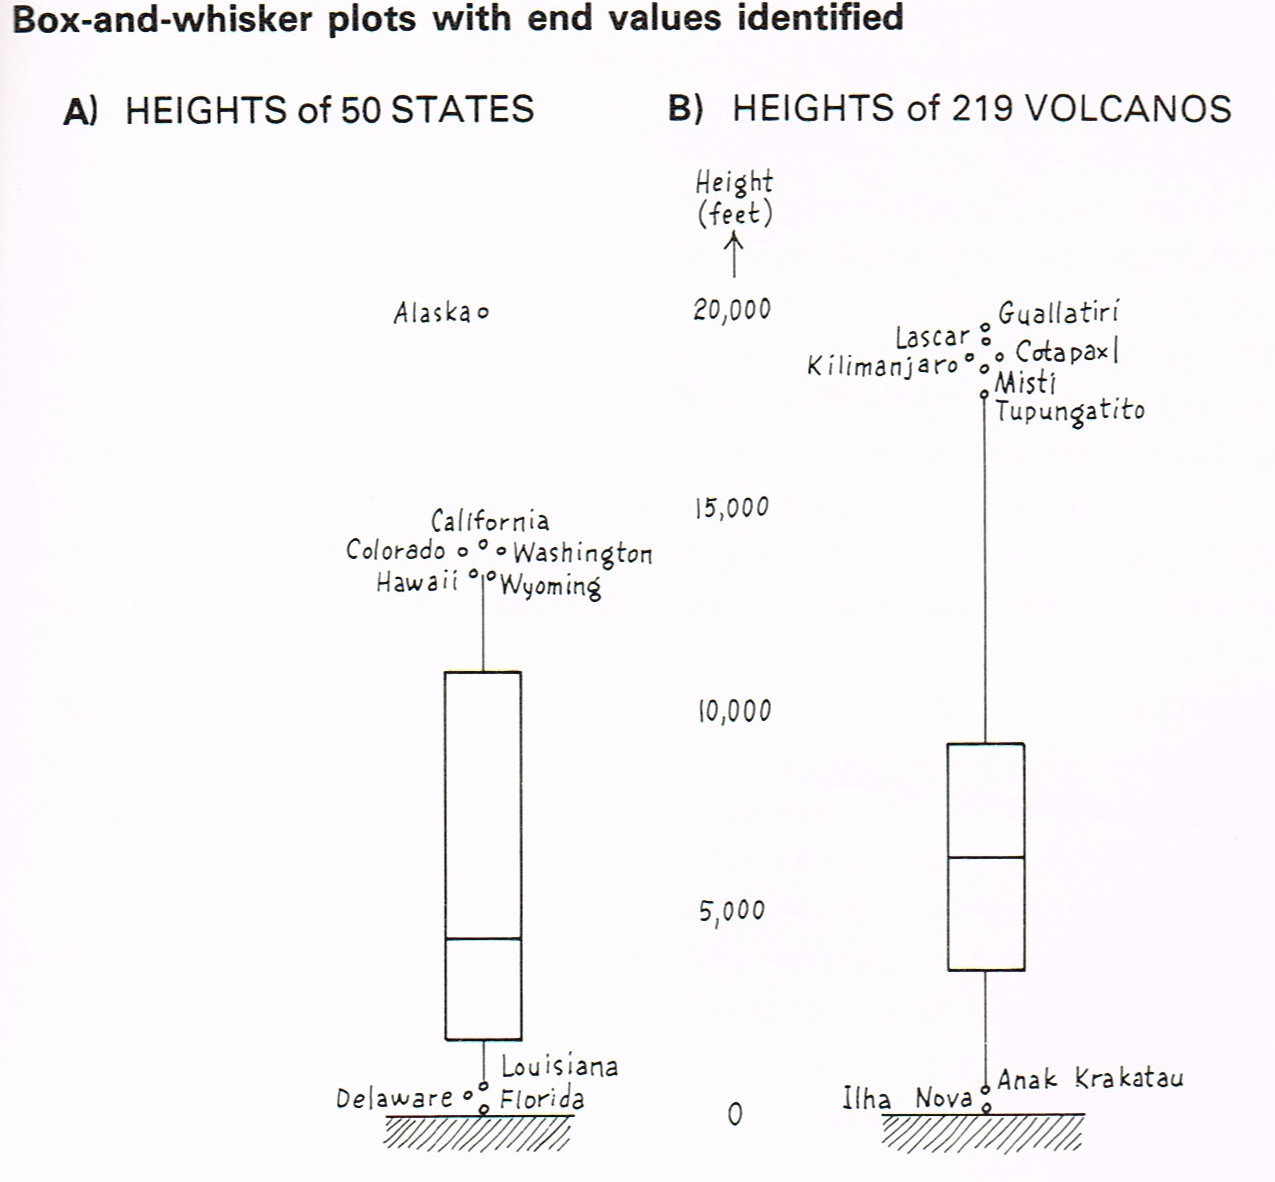
\includegraphics{figs/boxplot.png}
\caption{Tukey's 1977 example of the box plot (exhibit 6 of chapter 2 from
Exploratory Data Analytics\cite{tukey77e}) illustrates how the box plot shows
the distribution of topology of states and
the distribution of volcanos. The strength of the box and whisker is that the
reader can quickly compare the two distributions and learn, for example, that
volcanos tend to span a shorter range of average heights, but that the extremes
are much further from the center. Essentially, the distributions act as
references for the other displayed distributions.}
\label{fig:boxplot}
\end{figure}

In Tukey's introduction to the boxplot \cite{tukey77e}, shown in
figure~\ref{fig:boxplot}, the box and whisker plot takes the distributional information of a histogram and encodes the state heights between the
25th and 75th percentiles as a box, the median height as a line cutting across
the heights, and the extreme state heights as lines coming out of the
boxes. While a histogram would also show that the distribution of state heights has a fat right tail,
the power of the box and whisker plot is in encoding this information such that
it's trivial to compare to it's neighboring distribution of volcano
heights because they can share the Y-axis. As the number of distributions grow,
this technique becomes invaluable because the number of histograms that can be
placed next to each other or overlayed as pdfs can quickly become
unweildy.  Many others authors have kept the basic structure of the boxplot,
but exploited the structure to convey more information about the data. Authors used
different quantile levels \cite{Hyndman}s or measures or extremes\cite{Frigge,
carter}, proposed assymetric whiskers \cite{Rousseuw}, and otherwise incorporated skewness, kurtosis, and other descriptive distributional statsics \cite{ Aslam, choon, Marmelejo}.


\begin{figure}
%%\includegraphic{Mcgill} #annottate figure with highlighted line for the notches!
\label{fig:notched}
\end{figure}
The box-plot was then expanded out from descriptive statistics to facilitatting
inferential deduction through the notched boxplot. \cite{mcgill1978} The notched boxplot
arose as an expansion of indicating sample size through the width of the box,
which is a technique that only works well for relatively small sample sizes (\<
1000), at larger scales the widths are about equal. Instead, notches, as seen
in Figure~\ref{fig:notched}, are used to indicate the confidence level of the
median for that box. The medians are statistically different from each other at
the 95\% confidence level if the notches do not overlap. In
Figure~\ref{fig:notched}, all the notches overlap %%annotate figure with what
%%overlapping region means
and so the difference in telephone bills is not-significant, but there's a
statistically significant difference between the 11-15 and over 15 groups. Notches may extend
beyond the box edges, and sometimes the width technique is incorporated back
into the notched boxpplot such that the confidence can be grounded in sample
size. The notches in Figure~\ref{fig:notched} are computed assuming a gaussian
distribution, but many authors \cite{x,y,z} discuss ways to compute notches for
non-gaussian distributions. 

\begin{figure}
%%two figs a and b with a shared caption...
%%\includegraphics{benjamini}
\label{fig:histplot}
\label{fig:vase}
\end{figure}

Because the box-plot does not give any indication of how data is distributed
inside the box or along the whiskers, the histplot and vaseplot were introduced to indicate
the density of the data\cite{benjamini1988}. As shown in
Figure~\ref{fig:histplot} the histplot seperates the box
into  5 bins and scales the width of that section of the box based on the
number of values in that bin; it's essentially a rotated histogram. The
vaseplot, shown in Figure~\ref{fig:vase} removes the bins and is instead based
on the estimated density at that point in the data. The specific shape is
dependent on what sort of density estimation method is used, such as kernal
estimation or nearest neighbor estimation \cite{chambers1983}. The
violinplot \cite{hintz1998} expands this concept further by representing the
width using the density-trace method proposed by Chambers
et. al \cite{chambers1983}%%is density trace the same as a pdf? 





%letter value plots


%bagplots->

\begin{figure}
\includegraphics{figs/countour_weather.png}
\label{fig:countour}
\end{figure}
Countour Boxplots \cite{whitaker13} are an extension of boxplots that tries to better encapsulate outliers. Box plots inherently clip the uncertainity they show to some upper and lower band, 
creating a somewhat bounding envelope for the function that looks fairly regular when aggregated. Countour boxplots aim instead to capture the variablity of the uncertainity by trading in descripting
statistics for a measure called band depth. Each ensemble members band depth is computed as sum of the probabilities that the observations in any given ensemble fall within the max-min envelope defined by any two other ensembles. The bands are then sorted by band depth such that the median is the ensemble with about 50\% of its members withen all envelopes formed by other bands (so most centered). Outer bands are chosen according to the task at hand. In \cite{whitaker13}, they apply the countour boxplots to temperature visualizations. %
The authors argue that countour boxplots are an improved visual idiom over the traditional spagehttie plots seen in \ref{fig:countour} because as seen in (fig), the spagehetti plots get nosy as the number of plots increase and so it's hard to tease out specific patterns. Instead in (fig3), the authors remove most of the bands and instead visualize an outliser envelope(light gray) and a more central envelope(dark gray). It retains much of the information of the spagethhit, but removes the visual noise of the lines.  
